\section{Undersampling}
\subsection{Undersampling Data Set}
Undersampling is a technique to deal with class imbalance, as introduced in \cite{bloem2020methology1}. This simple approach reduces class imbalance by excluding instances from the majority class. The majority class is identified and randomly chosen instances of majority class are excluded to match the number of instances of the minority class. This is done recursively till all classes have an equal distribution. The resulting dataset is visualized in figure \ref{fig:undersampling_class_distribution}.

% on the left before, on the right after
\begin{figure}[h]
    \centering
    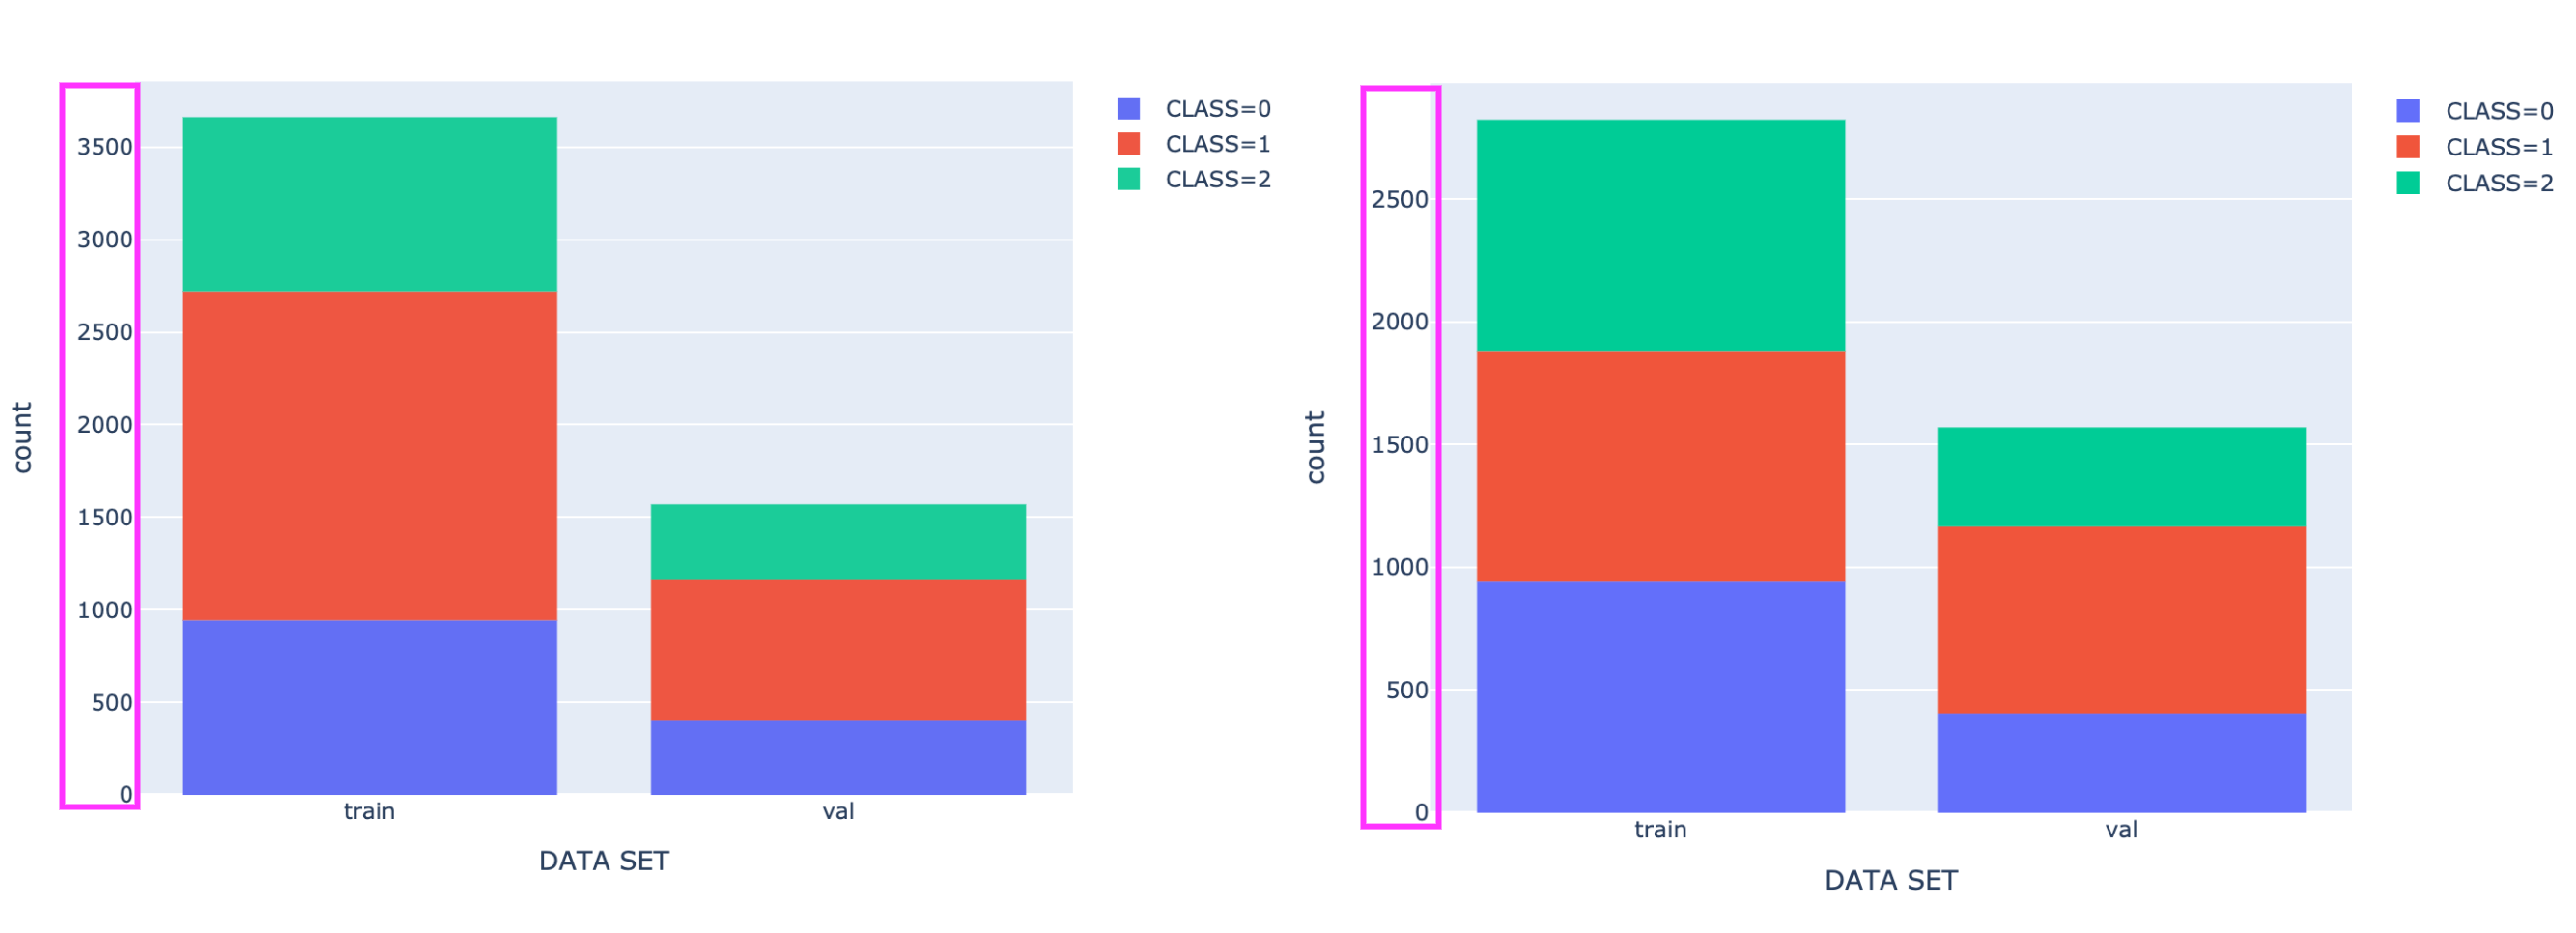
\includegraphics[width=\linewidth]{figures/undersampling/distribution_classes_before_after.png}
    \caption{Class distribution after undersampling. On the left before, on the right after. Note that the y-axis is scaled to the biggest dataset. Therefore, before and after are not shown on the same scale}
    \label{fig:undersampling_class_distribution}
\end{figure}

\subsection{Results on Validation Set} 
The CNN was trained three times with the undersampled data-set. The results, as can be seen in figure \ref{fig:under_val}, show no significant performance difference in both precision and recall compared to the baseline. The precision is in between a range of 0.80 to 0.82 in the baseline and training using the undersampled data-set with one outlying result which yields a result of 0.83. Both recall results are also in the same range from 0.78 to 0.80 except for the one outlying result which achieves a result of 0.82. 

\begin{figure}[!ht]
    \centering
    \subfloat[Precision]{\label{fig:under_val_a}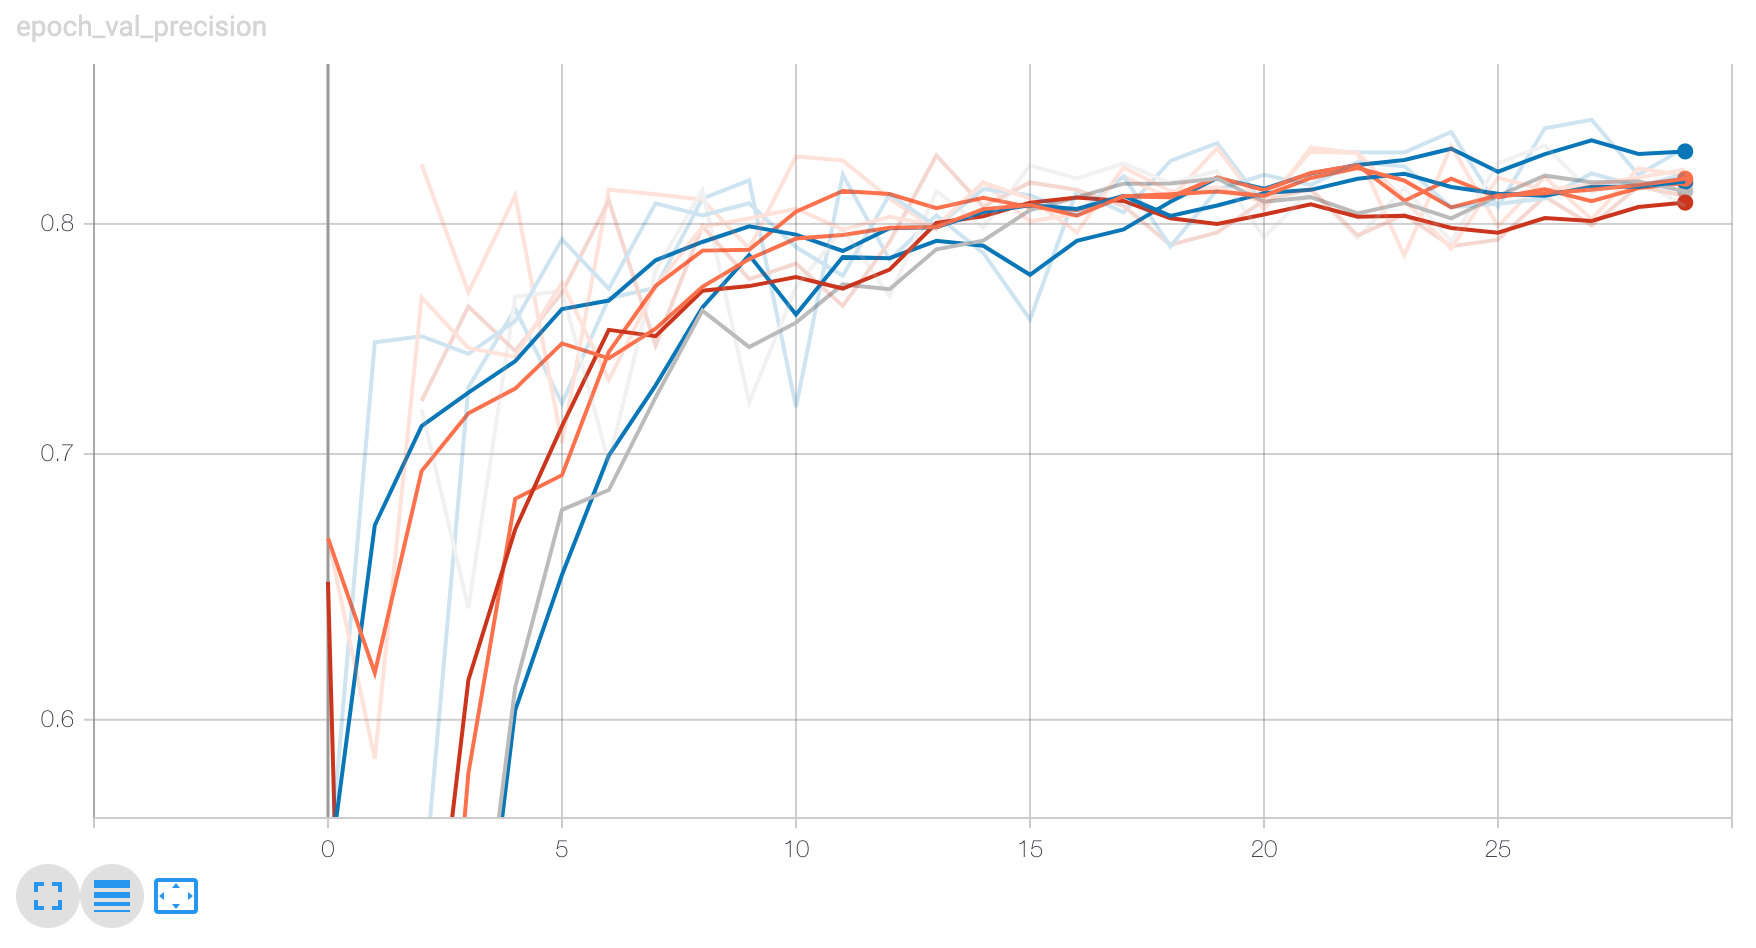
\includegraphics[width=0.89\linewidth]{figures/undersampling/val_precision.png}}
    \par\medskip
    \centering
    \subfloat[Recall]{\label{fig:under_val_b}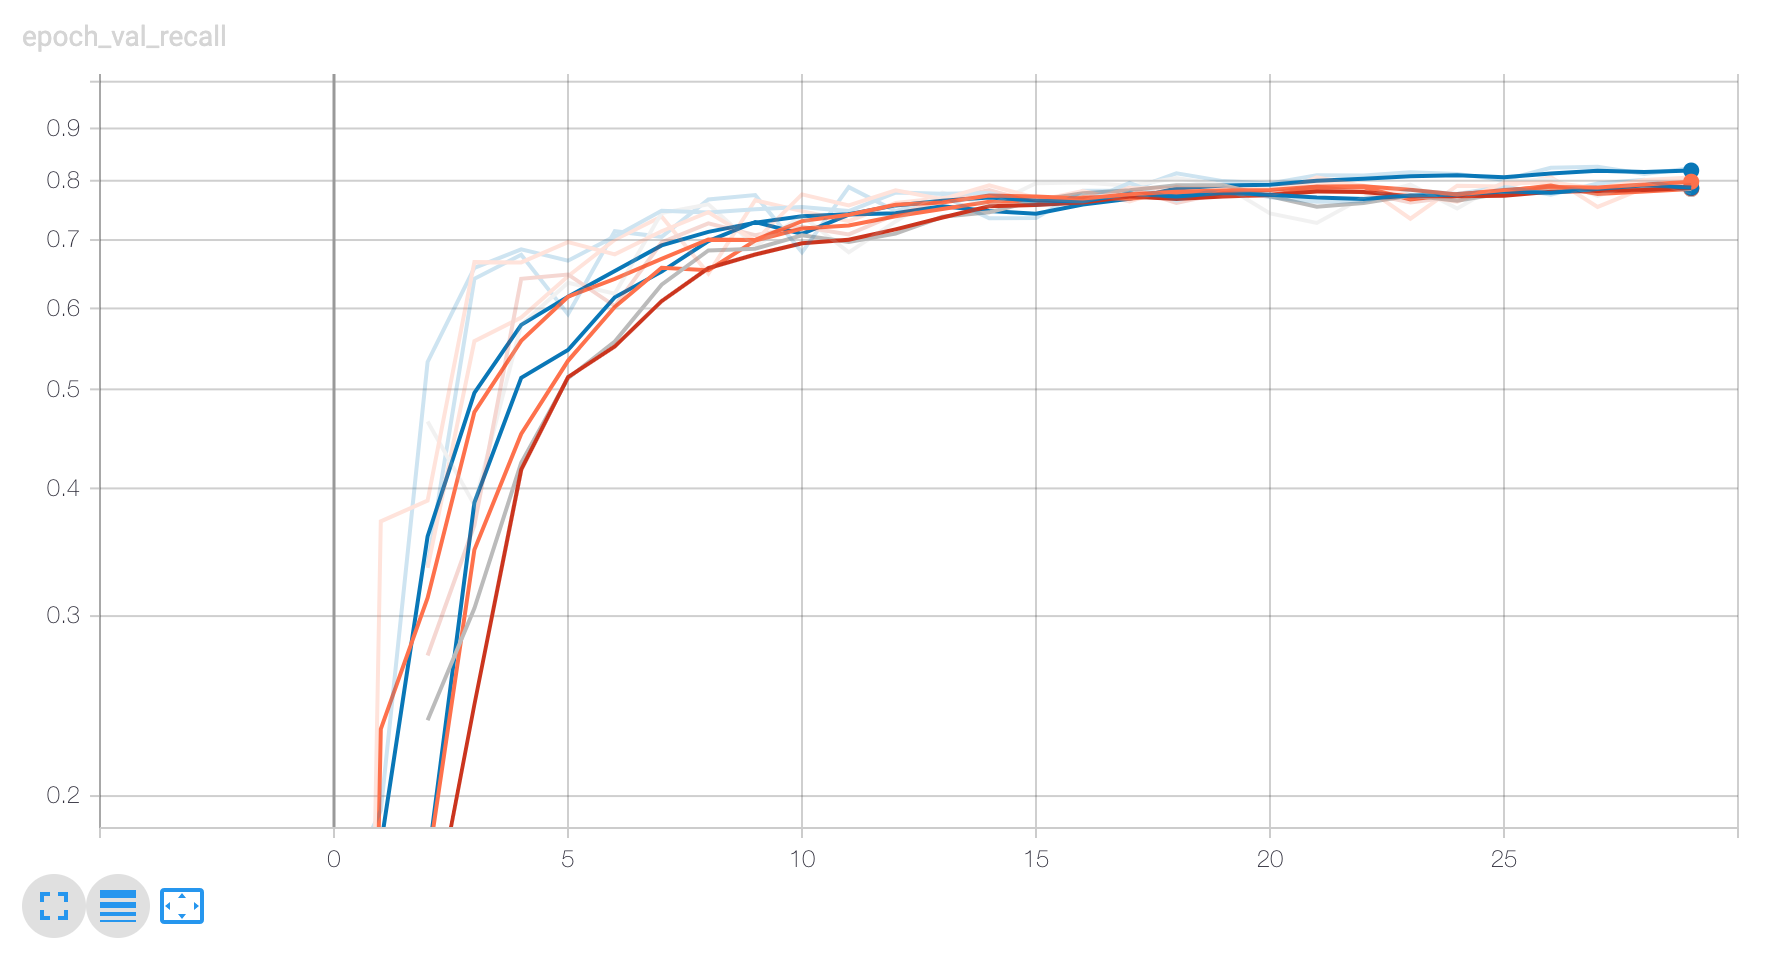
\includegraphics[width=0.89\linewidth]{figures/undersampling/val_recall.png}}
    \par\medskip
  \caption{Undersampling on Validation Set. The baseline and undersampling results are not clearly distinguishable which indicates no clear improvement or worsening.}
  \label{fig:under_val}
\end{figure}

\subsection{Results on Test Set}

\begin{equation}
Precision = 0.6770
\end{equation}
\begin{equation}
Recall = 0.6651
\end{equation}

No performance increase is achieved using undersampling. The differences on the validation set were thought to be due some randomness as the baseline also achieves different but very similar results. However, the results on the test set reveal that undersampling actually performs slightly worse than the baseline. \\
Reasons could be that we specifically made sure that the CNN is not overfitting. Undersampling lead to less training images which could have effected the overall results in a negative way. If the CNN would have overfitted with the original training set, we could have seen a positive result because the class imbalance, which would have likely lead to overfitting as can be seen in the oversampling chapter, would be neglected.   